% Include header.tex with configuration
%**********************************************************************
%* Niets toevoegen aan dit bestand zonder toestemming van uw promotor *
%**********************************************************************
\documentclass[12pt,a4paper,oneside]{book}

%%%%%%%%%%%%%%%%%%%%%%%%%%%%%%%%%%%%%%%%%%%%%%%%%%%%%%%%%%%%%%%%%%%%%%%%%%%%%%%%%%
%% Volgende regel activeren voor eReader output:
%\usepackage[papersize={130mm,180mm},margin=2mm]{geometry}

%% Volgende regel activeren voor A4 output (bovenstaande terug afzetten)
\usepackage{a4wide} % Iets meer tekst op een bladzijde
%%%%%%%%%%%%%%%%%%%%%%%%%%%%%%%%%%%%%%%%%%%%%%%%%%%%%%%%%%%%%%%%%%%%%%%%%%%%%%%%%%

%% Packages %%
\usepackage{a4wide}                     % Iets meer tekst op een bladzijde
\usepackage[dutch]{babel}               % Voor nederlandstalige woordsplitsing (en chapter hoofdingen)
\usepackage{amsmath}                    % Uitgebreide wiskundige mogelijkheden
\usepackage{url}                        % Om urls te verwerken
\usepackage{graphicx}                   % Om figuren te kunnen verwerken
\usepackage[latin1]{inputenc}           % Om niet ascii karakters te kunnen typen
\usepackage[pagebackref=true]{hyperref}
\usepackage{listings}                   % improve the code environments
%\usepackage{lmodern}
%\usepackage[T1]{fontenc}
\usepackage{textcomp}
\usepackage{pdfpages}                   % Om pdf documenten in te kunnen voegen (titelpagina)
\usepackage{lipsum}                     % Om lorem ipsum in te voegen
\usepackage{sty/eukdate}                % Om de datum in te voegen 
\usepackage[DoggensLenny]{sty/fncychap} % Added for nicer formatting: (kaders rond titels)
\usepackage{fix-cm}
\usepackage{parskip}                    % Geen inspringing aan het begin van een alinea
%\usepackage{sectsty}
\usepackage{mdwlist}
\usepackage{sty/eukdate}                % Om data in te voegen
\usepackage{caption}
\usepackage{float}                      % Om afbeelding geforceerd op een plek te plaatsten met 'H' parameter
\restylefloat{figure}
\usepackage{multirow}                   % Weergave van complexere tabellen
\usepackage[scaled]{sty/inconsolata}    % Instelling lettertype
\usepackage{verbatim}

\hypersetup{                            % Markup for links in text, final versie enkel met zwarte links!!  %%
    colorlinks = false,                 %false=rode kaders rond tekst, true=links in de tekst zelf in kleur
    linkcolor = black,
    anchorcolor = black,
    citecolor = blue,
    filecolor = black,
    urlcolor = black
}

\renewcommand*\familydefault{\sfdefault}                        % Only if the base font of the document is to be sans serif
%\allsectionsfont{\usefont{OT1}{phv}{bc}{n}\selectfont}
  
\hyphenpenalty=5000                                             % Minder snel woorden splitsen
  \tolerance=1000

%% Custom commands %%
\newcommand{\npar}{\par \vspace{2.3ex plus 0.3ex minus 0.3ex}}  % Enkele mm vertikale ruimte openlaten
\newcommand{\ntpar}{\par \vspace{1.3ex plus 0.3ex minus 0.3ex}}
\newcommand{\nhpar}{\par \vspace{4.3ex plus 0.3ex minus 0.3ex}}

\newcommand{\HRule}{\rule{\linewidth}{0.5mm}}                   % Horizontale lijn

\setcounter{tocdepth}{2}                                        % weergeven tot subsection in table of contents

% \usepackage[final]{sty/TODO}           %TODO package (build error als er nog een todo in het document staat)
%\usepackage[silent]{sty/TODO}           %TODO package (geen output, om een tussentijdse draft zonder de 'todos' te maken)
\usepackage{sty/TODO}                    %TODO package (standaard modus)


\usepackage{eso-pic}
\newcommand\BackgroundPic{%
\put(0,0){%
\parbox[b][\paperheight]{\paperwidth}{%
\vfill
\centering
% 
\includegraphics[width=\paperwidth,height=\paperheight]{figures/titelpagina_ap_lowestres.jpg}
% 
\includegraphics[width=\paperwidth,height=\paperheight]{figures/titelpagina_ap_lowres.jpg}

\includegraphics[width=\paperwidth,height=\paperheight]{figures/titelpagina_ap_mediumres.jpg}

\vfill
}}\hfill
}

\newcommand\BackgroundPicAP{%
\put(220,-372){%
\parbox[b][\paperheight]{\paperwidth}{%
\vfill
\centering

\includegraphics[width=0.44\paperwidth,height=0.075\paperheight,keepaspectratio]{figures/AP.png}
\vfill
}}
\hfill
}

%*************************************************************************************
%* Plaats eventuele extra toegevoegde packages hier (na toestemming van uw promotor) *
%*************************************************************************************





% Use colors for corporate design
% Farbpalette A
\definecolor{blau_1a}{RGB}{93,133,195}
\definecolor{blau_2a}{RGB}{0,156,218}
\definecolor{gruen_3a}{RGB}{80,182,149}
\definecolor{gruen_4a}{RGB}{175,204,80}
\definecolor{gruen_5a}{RGB}{221,223,72}
\definecolor{orange_6a}{RGB}{255,224,92}
\definecolor{orange_7a}{RGB}{248,186,60}
\definecolor{rot_8a}{RGB}{238,122,52}
\definecolor{rot_9a}{RGB}{233,80,62}
\definecolor{lila_10a}{RGB}{201,48,142}
\definecolor{lila_11a}{RGB}{128,69,151}

% Farbpalette B
\definecolor{blau_1b}{RGB}{0,90,169}
\definecolor{blau_2b}{RGB}{0,131,204}
\definecolor{gruen_3b}{RGB}{0,157,129}
\definecolor{gruen_4b}{RGB}{153,192,0}
\definecolor{gruen_5b}{RGB}{201,212,0}
\definecolor{orange_6b}{RGB}{253,202,0}
\definecolor{orange_7b}{RGB}{245,163,0}
\definecolor{rot_8b}{RGB}{236,101,0}
\definecolor{rot_9b}{RGB}{230,0,26}
\definecolor{lila_10b}{RGB}{166,0,132}
\definecolor{lila_11b}{RGB}{114,16,133}

\newglossary[sylg]{symbolslist}{syi}{syo}{Nomenclature}
\makeglossaries

\begin{acronym}[ACRONYM] 
% Change the word ACRONYM above to change the acronym column width.
% The column width is equals to the width of the word that you put.
% Read the manual about acronym package for more examples:
%   http://linorg.usp.br/CTAN/macros/latex/contrib/acronym/acronym.pdf
  \acro{AJAX}{Asynchronous JavaScript and XML}
  \acro{BAST}{Bug Report Analysis and Search Tool}
  \acro{BTT}{Bug Report Tracker Tool}
  \acro{BRN}{Bug Report Network}
  \acro{CCB}{Change Control Board}
\end{acronym}

\begin{document}

\begin{titlepage}
	\centering
    \vspace*{0.5 cm}
    \includegraphics[scale = 0.5]{./img/logo_ucleuvenlimburg_rgb.png}\\[1cm]% University Logo
    %\textsc{\LARGE \naamschool}\\[2.0 cm]	% University Name
    %\textsc{\huge \naamschool}\\[2.0 cm]	% University Name
    \textsc{\Huge	 \naamschool}\\[2.0 cm]	% University Name

	%\textsc{\Large \coursecode}\\[1.5 cm]				% Course Code en
\textsc{\huge \coursecode}\\[1.5 cm]				% Course Code en
%\textsc{\Huge \coursecode}\\[1.5 cm]				% Course Code en

	%\textsc{\Large \info}\\[0.5 cm]				% Course Name
\textsc{\huge \info}\\[0.5 cm]				% Course Name
%\textsc{\Huge \info}\\[0.5 cm]				% Course Name
	% Title
	%\HRule \\[0.4cm]
\HRule \\[0.6cm]
	%\rule{\linewidth}{0.2 mm} \\[0.4 cm]
	{\huge \bfseries \thetitle}\\[0.4cm]
	%\rule{\linewidth}{0.2 mm} \\[1.5 cm]
	\HRule \\[1.5cm]


	% Author and supervisor
	\begin{minipage}{0.4\textwidth}
		\begin{flushleft} \large
			\emph{Auteur:}\\
			Filip Vanden Eynde
			\end{flushleft}
			\end{minipage}~
			\begin{minipage}{0.4\textwidth}
			\begin{flushright} \large
			\emph{Student Number:} \\
			r0363898									% Your Student Number
		\end{flushright}
	\end{minipage}\\[3 cm]  %\\[2 cm]
	%\end{minipage}
	%\vfill

	% Bottom of the page
    %{\large januari, 2016}
	
	%{\large \MONTH , \YEAR}%\\[2 cm]

	{\large \today}%\\[2 cm]

	\vfill
	
\end{titlepage}
%%%%%%%%%%%%%%


\makethesistitle

% Start with roman page numbering
\pagenumbering{Roman}

% Comment out the following two lines before printing your final document
\listoftodos
\newpage

% Print table of contents
\tableofcontents

\newpage

% Print list of figures
\listoffigures

\newpage

% Print list of tables
\listoftables

\newpage

% Define custom style for glossaries
\newglossarystyle{mystyle}{%
  % full stop after every description
	\renewcommand*{\glspostdescription}{}%
	% put the glossary in a longtable environment:
  % left alignment, no white in front und three columns
	\renewenvironment{theglossary}{\begin{longtable}[l]{@{}lcl}}{\end{longtable}}
	% have nothing after \begin{theglossary}:
	\renewcommand*{\glossaryheader}{}%
  % uncomment following line if you want headings
	% \renewcommand*{\glossaryheader}{\bfseries Symbol & \bfseries Unit & \bfseries Description \endhead}%
	% have nothing between glossary groups (next two commands):
	\renewcommand*{\glsgroupheading}[1]{}%
	% Suppress the vertical gap at the start of each group
	\renewcommand*{\glsgroupskip}{}%
	% set how each entry should appear:
	\renewcommand*{\glossaryentryfield}[5]{%
		\glstarget{##1}{##2}	% Name
		& ##4					        % Symbol
		& ##3					        % Description
		% & ##5					      % Page list
		\\% end of row
	}%
	% Sub entries treated the same as level 0 entries:
	\renewcommand*{\glossarysubentryfield}[6]{%
		\glossaryentryfield{##2}{##4}{##3}
	}%
}

% Print acronyms
\printglossary[type=acronym, title=Acronyms, toctitle=Acronyms, style=mystyle]

% Print list of symbols
\printglossary[type=symbolslist, style=mystyle]
\newpage

% Save current value of roman page number
\newcounter{romanpagenumbers}
\setcounter{romanpagenumbers}{\value{page}}

% Change to arabic page numbers
\pagenumbering{arabic}

% --- Equations ---
\chapter{Equations}

Equation for extraterrestrial radiation with \gls{I0}, \gls{SC}, \gls{n}, \gls{L}, \gls{delta} and \gls{HSR}.

\begin{equation}
  \glsentrytext{I0} = \frac{24}{\pi} \glsentrytext{SC} \left[1+0,034\cos\left(\frac{360\glsentrytext{n}}{365}\right)\right](\cos \glsentrytext{L} \cos \glsentrytext{delta} \sin \glsentrytext{HSR} + \glsentrytext{HSR} \sin \glsentrytext{L} \sin \glsentrytext{delta})
\end{equation}

Equation for average wind power.

\begin{equation}
	\overline P_w = \frac{c_1}{T} \int_0^T v_w^3\,dt \ne c_1 \left(\frac{1}{T}\int_0^T v_w\,dt\right)^3 = c_1 \cdot \overline{v}_w^3.
\end{equation}

% --- Acronyms ---
\chapter{Acronyms}

Use package \href{ftp://ftp.dante.de/tex-archive/macros/latex/contrib/glossaries/glossariesbegin.pdf}{glossaries}.

Lorem ipsum dolor sit amet, consectetuer adipiscing elit \textbf{\gls{CO2} for the first time}, sed diam nonummy nibh euismod tincidunt ut laoreet dolore magna aliquam erat volutpat. Ut wisi enim ad minim veniam, quis nostrud exerci tation ullamcorper suscipit lobortis nisl ut aliquip ex ea commodo consequat. Duis autem vel eum iriure dolor in hendrerit in vulputate velit esse molestie consequat \textbf{\gls{CO2} for the second time}, vel illum dolore eu feugiat nulla facilisis at vero eros et accumsan et iusto odio dignissim qui blandit praesent luptatum zzril delenit augue duis dolore te feugait nulla facilisi. Nam liber tempor cum soluta nobis eleifend option congue nihil imperdiet doming id quod mazim placerat facer possim assum. Typi non habent claritatem insitam; est usus legentis in iis qui facit eorum claritatem. 

Lorem ipsum dolor sit amet, consectetuer adipiscing elit \textbf{\gls{NEDC} for the first time}, sed diam nonummy nibh euismod tincidunt ut laoreet dolore magna aliquam erat volutpat. Ut wisi enim ad minim veniam, quis nostrud exerci tation ullamcorper suscipit lobortis nisl ut aliquip ex ea commodo consequat. Duis autem vel eum iriure dolor in hendrerit in vulputate velit esse molestie consequat \textbf{\gls{NEDC} for the second time}, vel illum dolore eu feugiat nulla facilisis at vero eros et accumsan et iusto odio dignissim qui blandit praesent luptatum zzril delenit augue duis dolore te feugait nulla facilisi. Nam liber tempor cum soluta nobis eleifend option congue nihil imperdiet doming id quod mazim placerat facer possim assum. Typi non habent claritatem insitam; est usus legentis in iis qui facit eorum claritatem. 

Lorem ipsum dolor sit amet, consectetuer adipiscing elit \textbf{\gls{D} for the first time}, sed diam nonummy nibh euismod tincidunt ut laoreet dolore magna aliquam erat volutpat. Ut wisi enim ad minim veniam, quis nostrud exerci tation ullamcorper suscipit lobortis nisl ut aliquip ex ea commodo consequat. Duis autem vel eum iriure dolor in hendrerit in vulputate velit esse molestie consequat \textbf{\gls{D} for the second time}, vel illum dolore eu feugiat nulla facilisis at vero eros et accumsan et iusto odio dignissim qui blandit praesent luptatum zzril delenit augue duis dolore te feugait nulla facilisi. Nam liber tempor cum soluta nobis eleifend option congue nihil imperdiet doming id quod mazim placerat facer possim assum. Typi non habent claritatem insitam; est usus legentis in iis qui facit eorum claritatem. 

% --- Simple citations ---
\chapter{Citations}

This could be a sentence from a book.\cite{wagner2010}

% --- Page numbering ---
\chapter{Page numbering}

The template consists of four parts. 

The first part includes the title and second page and doesn't have any page numbers. 

The second part consists of the table of contents, list of figures, list of tables, acronyms and symbols. It has roman page numbers and starts at \textbf{I}. 

The third part contains the main content. It has arabic page numbers and starts at \textbf{1}. 

The fourth and last part includes the bibliography. It has roman page numbers and continues the counting from part two.

The title and second page don't have any page numbers. It is therefore important to start with the roman page numbering below the command \textbf{\textbackslash makethesistitle}. Otherwise \LaTeX{} will throw warnings like

\begin{verbatim}
pdfTeX warning (ext4): 
destination with the same identifier (name{page.}) has been already used,
duplicate ignored
\end{verbatim}

% --- Complex tables ---
\chapter{Table}

Table \ref{tab:inflation} shows a simple example with footnotes.

\ctable[
	cap = Economic situation in Austria,
	caption = Economic situation in Austria \cite{verbraucher2011, prognose2011},
	label	= tab:inflation,
	pos = htb
	]{lrr}
	{
		\tnote[1]{Consumer price index}
		\tnote[2]{Index 1990 = 100}
		\tnote[3]{Forecast value}
	}
	{\FL	Year			& Inflation rate in \%\tmark[1]		& Price trend\tmark[2]
	\ML		2000			& 2,3								& 125,7
	\NN		2001			& 2,7								& 129,1
	\NN		2002			& 1,8								& 131,5
	\NN		2003			& 1,3								& 133,2
	\NN		2004			& 2,1								& 136,0
	\NN		2005			& 2,3								& 139,1
	\NN		2006			& 1,5								& 141,2
	\NN		2007			& 2,2								& 144,3
	\NN		2008			& 3,2								& 148,9
	\NN		2009			& 0,5								& 149,6
	\NN		2010			& 1,9								& 152,4
	\NN 	2011\tmark[3]	& 2,1								& 155,6
	\NN		2012\tmark[3]	& 1,8								& 158,4
	\LL}

\newpage

Table \ref{tab:data_imiev} shows a more complex example

\ctable[
	caption = Technical data of the Mitsubishi i-MiEV \cite{imiev_daten},
	cap = Technical Data of the Mitsubishi i-MiEV,
	label	= tab:data_imiev,
	pos = htb
	]{llr}
	{\tnote[1]{Data measured in NEDC}}
	{\FL Description & Specification & Value
		\ML \multirow{4}*{Dimensions} & Length & 3475 mm
		\NN & Width & 1475 mm
		\NN & Height & 1610 mm
		\NN & Wheel base & 2550 mm
		\ML \multirow{5}*{Load capacity} & Luggage space & 227 / 860 liters
		\NN & Curb weight & 1110 kg
		\NN & Permissible maximum weight & 1450 kg
		\NN & Payload & 340 kg
		\NN & Seats & 4 People
		\ML \multirow{3}*{Driving characteristics} & Energy consumption & 135 Wh/km
		\NN & Range & 150 km\tmark[1]
		\NN & max. Velocity & 130 km/h
		\ML \multirow{5}*{Battery data} & Nominal voltage & 330 V
		\NN & Electric charge & 50 Ah
		\NN & Theoret. energy & 16500 Wh
		\NN & Mass & 165 kg
		\NN & Energy density & 100 Wh/kg
		\ML \multirow{3}*{Motor data} & Typ & Permanent Synchronous Motor
		\NN & Nominal power & 35 kW
		\NN & max. Torque & 180 Nm
		\LL}

% --- To-do notes ---
\chapter{To-do notes}

Very useful while writing the thesis. Don't forget to delete them before printing the final copy.

Lorem ipsum dolor sit amet, consectetuer adipiscing elit. Aenean commodo ligula eget dolor. Aenean massa. Cum sociis natoque penatibus et magnis dis parturient montes, nascetur ridiculus mus. Donec quam felis, ultricies nec, pellentesque eu, pretium quis, sem. Nulla consequat massa quis enim. Donec pede justo, fringilla vel, aliquet nec, vulputate eget, arcu. In enim justo, rhoncus ut, imperdiet a, venenatis vitae, justo. Nullam dictum felis eu pede mollis pretium. Integer tincidunt. Cras dapibus. Vivamus elementum semper nisi. Aenean vulputate eleifend tellus. Aenean leo ligula, porttitor eu, consequat vitae, eleifend ac, enim. Aliquam lorem ante, dapibus in, viverra quis, feugiat a, tellus. Phasellus viverra nulla ut metus varius laoreet. Quisque rutrum. Aenean imperdiet. Etiam ultricies nisi vel augue. Curabitur ullamcorper ultricies nisi. Nam eget dui. Etiam rhoncus. Maecenas tempus, tellus eget condimentum rhoncus, sem quam semper libero, sit amet adipiscing sem neque sed ipsum. Nam quam nunc, blandit vel, luctus pulvinar, hendrerit id, lorem. Maecenas nec odio et ante tincidunt tempus. Donec vitae sapien ut libero venenatis faucibus. Nullam quis ante. Etiam sit amet orci eget eros faucibus tincidunt. Duis leo. Sed fringilla mauris sit amet nibh. Donec sodales sagittis magna.

\todo[inline]{Translate text to english}

Lorem ipsum dolor sit amet, consectetuer adipiscing elit. Aenean commodo ligula eget dolor. Aenean massa. Cum sociis natoque penatibus et magnis dis parturient montes, nascetur ridiculus mus. Donec quam felis, ultricies nec, pellentesque eu, pretium quis, sem. Nulla consequat massa quis enim. Donec pede justo, fringilla vel, aliquet nec, vulputate eget, arcu. In enim justo, rhoncus ut, imperdiet a, venenatis vitae, justo. Nullam dictum felis eu pede mollis pretium. Integer tincidunt. Cras dapibus. Vivamus elementum semper nisi. Aenean vulputate eleifend tellus. Aenean leo ligula, porttitor eu, consequat vitae, eleifend ac, enim. Aliquam lorem ante, dapibus in, viverra quis, feugiat a, tellus. Phasellus viverra nulla ut metus varius laoreet. Quisque rutrum. Aenean imperdiet. Etiam ultricies nisi vel augue. Curabitur ullamcorper ultricies nisi. Nam eget dui. Etiam rhoncus. Maecenas tempus, tellus eget condimentum rhoncus, sem quam semper libero, sit amet adipiscing sem neque sed ipsum. Nam quam nunc, blandit vel, luctus pulvinar, hendrerit id, lorem. Maecenas nec odio et ante tincidunt tempus. Donec vitae sapien ut libero venenatis faucibus. Nullam quis ante. Etiam sit amet orci eget eros faucibus tincidunt. Duis leo. Sed fringilla mauris sit amet nibh. Donec sodales sagittis magna.

\todo[inline]{Something else to do}

% --- Images side by side ---
\chapter{Images}

Figure \ref{fig:mitsubishi_imiev} shows two pictures side by side with one caption.

\begin{figure}[htb]
	\centering
	\subfloat{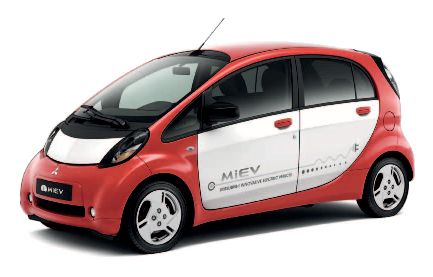
\includegraphics[width=80mm]{images/mitsubishi_imiev}}\hspace{10mm}
	\subfloat{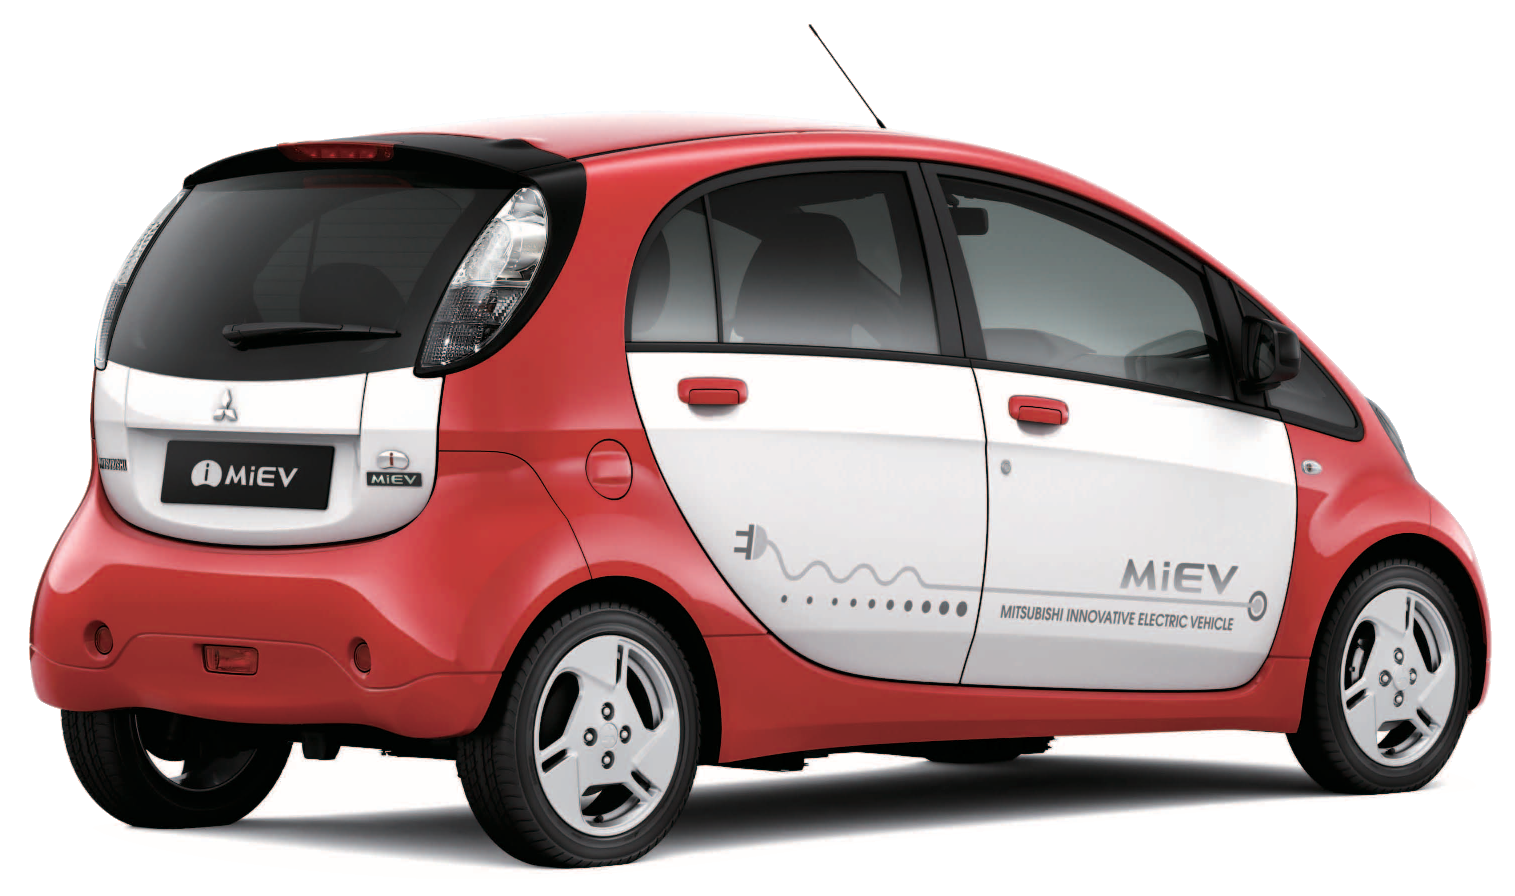
\includegraphics[width=80mm]{images/mitsubishi_imiev2}}
	\caption[The Mitsubishi i-MiEV]{The Mitsubishi i-MiEV \cite{mmd2010}}
	\label{fig:mitsubishi_imiev}
\end{figure}

% --- Bar chart ---
\chapter{Bar charts}

This chapter shows how to render a simple bar chart, a stacked bar chart and a grouped bar chart.

% --- Simple bar chart ---
\section{Simple bar chart}

Figure \ref{fig:new_ev} shows a simple bar chart.

\begin{figure}[htb] 
	\centering
	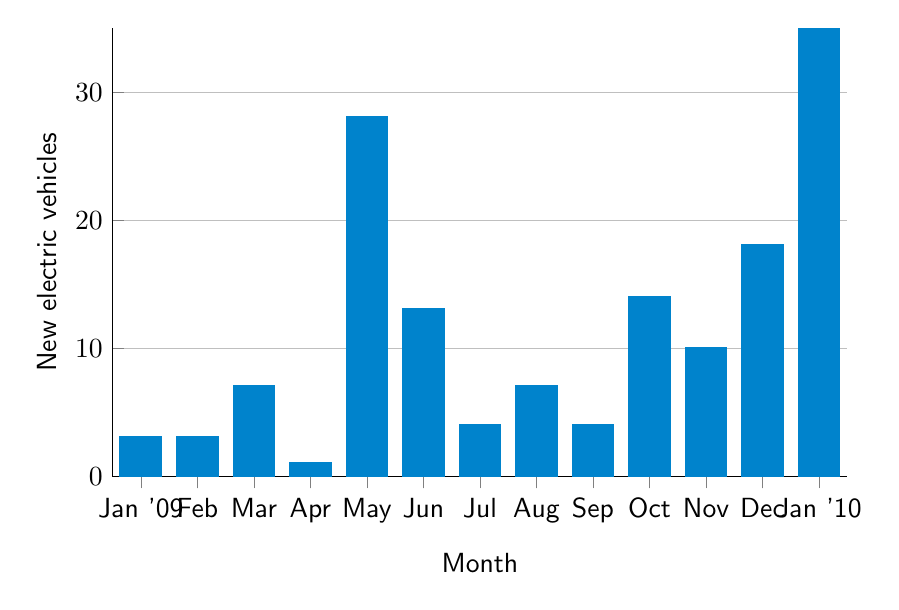
\begin{tikzpicture} 
		\begin{axis}[
			ybar,
			xlabel = Month,
			xmin = 0.5,
			xmax = 13.5,
			ymin = 0,
			ymax = 35,
			axis x line* = bottom,
			axis y line* = left,
			ylabel= New electric vehicles,
			width= 0.9\textwidth,
			height = 0.6\textwidth,
			ymajorgrids = true,
			bar width = 5mm,
			xticklabels = \empty,
			extra x ticks = {1,2,3,4,5,6,7,8,9,10,11,12,13},
			extra x tick labels = {Jan '09, Feb, Mar, Apr, May, Jun, Jul, Aug, Sep, Oct, Nov, Dec, Jan '10},
			]
			\addplot+[mark=none, blau_2b, very thick] coordinates {
				(1,3)
				(2,3)
				(3,7)
				(4,1)
				(5,28)
				(6,13)
				(7,4)
				(8,7)
				(9,4)
				(10,14)
				(11,10)
				(12,18)
				(13,35)
			};
		\end{axis} 
	\end{tikzpicture}
	\caption[New electric vehicles between Januar 2010 and Januar 2011]{New electric vehicles between Januar 2010 and Januar 2011 \cite{sa-neuzulassungen}}
	\label{fig:new_ev}
\end{figure}

\newpage

% --- Stacked bar chart ---
\section{Stacked bar chart}

Figure \ref{fig:energy_austria} shows a stacked bar chart. Data from  \href{http://www.e-control.at/de/statistik/strom/betriebsstatistik/jahresreihen}{Energy Control Austria}. Chart shows energy production from \gls{ROR}, Storage power plant, Thermal power station and Renewable energy.

\begin{figure}[htb] 
	\centering
	\begin{tikzpicture} 
		\begin{axis}[
			ybar stacked,
			xlabel= Year,
			ylabel = Energy in GWh,
			ymajorgrids = true,
			width = 0.9\textwidth,
			height = 0.5\textwidth,
			xmin = 1999.5,
			xmax = 2009.5,
			ymin = 0,
			ymax = 70000,
			axis x line* = bottom,
			axis y line* = left,
			xticklabels = none,
			extra x ticks = {2000, 2001, 2002, 2003, 2004, 2005, 2006, 2007, 2008, 2009},
			extra x tick labels = {2000, 2001, 2002, 2003, 2004, 2005, 2006, 2007, 2008, 2009},
			legend style = {at={(0.5, 1.025)}, anchor = south, legend columns = -1, draw=none, area legend},  
      area legend,
			scaled ticks = false,
			y tick label style = {/pgf/number format/use comma}
			]
			\addplot+[mark=none, fill=blau_2b, draw = blau_2b, bar width = 8mm] table[x=year, y=ror] {data/stacked-bar-chart.dat};
			\addplot+[mark=none, fill=lila_10b, draw = lila_10b, bar width = 8mm] table[x=year, y=storage] {data/stacked-bar-chart.dat};
			\addplot+[mark=none, fill=orange_6b, draw = orange_6b, bar width = 8mm] table[x=year, y=thermal] {data/stacked-bar-chart.dat};
			\addplot+[mark=none, fill=gruen_4b, draw = gruen_4b, bar width = 8mm] table[x=year, y=renewable] {data/stacked-bar-chart.dat};
			\legend{\gls{ROR}, Storage power plant, Thermal power station, Renewable energy}
		\end{axis} 
	\end{tikzpicture}
	\caption[Energy production in Austria]{Energy production in Austria \cite{econtrol2011}}
	\label{fig:energy_austria}
\end{figure}

\newpage

% --- Grouped bar chart ---
\section{Grouped bar chart}

Figure \ref{fig:co2_einsparung_wind} shows a grouped bar chart. some ref to co2 \gls{CO2}. Taken from \href{http://www.nachhaltigwirtschaften.at/edz_pdf/0646_windenergieanlagen.pdf}{Systemmodell zur Optimierung der Integration von Windenergieanlagen in Österreich und Deutschland} page 126

\begin{figure}[htb] 
	\centering
	\begin{tikzpicture} 
		\begin{axis}[
			ybar,
			xlabel = Year,
			% xticklabels = none,
			xtick=\empty,
			extra x ticks = {1,2,3,4,5},
			extra x tick labels = {2000,2005,2010,2015,2020},
			% xmin = 1,
			% xmax = 96,
			ymin = 0,
			ymax = 900,
			axis x line* = bottom,
			axis y line* = left,
			ylabel= \gls{CO2} savings in g \gls{CO2}/kWh,
			width= 0.9\textwidth,
			height = 0.5\textwidth,
			ymajorgrids = true,
			y tick label style = {/pgf/number format/use comma},
			bar width = 6mm,
			legend style = {at={(0.5, 1.025)}, anchor = south, legend columns = -1, draw=none, area legend},
			area legend,
			]
			\addplot+[mark=none, blau_2b, very thick] table[x=year, y=de] {data/grouped-bar-chart.dat};
			\addplot+[mark=none, gruen_4b, very thick] table[x=year, y=at] {data/grouped-bar-chart.dat};
			\legend{Germany, Austria}
		\end{axis} 
	\end{tikzpicture}
	\caption[CO$_2$ savings from wind turbines]{CO$_2$ savings from wind turbines in Germany and Austria \cite{auer06}}
	\label{fig:co2_einsparung_wind}
\end{figure}

% --- Pie chart ---
\chapter{Pie chart}

Figure \ref{fig:co2_wind} shows a pie chart.

\newcommand{\slice}[4]{
  \pgfmathparse{0.5*#1+0.5*#2}
  \let\midangle\pgfmathresult
  % slice
  \draw[thick] (0,0) -- (#1:1) arc (#1:#2:1) -- cycle;
  % outer label
  \node[label=\midangle:#4] at (\midangle:1) {};
  % inner label
  \pgfmathparse{min((#2-#1-10)/110*(-0.3),0)}
  \let\temp\pgfmathresult
  \pgfmathparse{max(\temp,-0.5) + 0.8}
  \let\innerpos\pgfmathresult
  \node at (\midangle:\innerpos) {#3};
}

	\begin{figure}[htb]
		\centering
		\begin{tikzpicture}[scale=3]
		\newcounter{a}
		\newcounter{b}
		\foreach \p/\t in {5/Shot break, 19/Rotor, 7/Gear + Generator, 18/remaining Housing, 20/Tower, 6/Power connection, 8/Basement, 3/Misc, 14/Operation}
		 {
		    \setcounter{a}{\value{b}}
		    \addtocounter{b}{\p}
		    \slice{\thea/100*360}
		          {\theb/100*360}
		          {\p\%}{\t}
		  }
		\end{tikzpicture}
		\caption[Break down of the CO$_2$ emissions of a wind turbine]{Break down of the CO$_2$ emissions of a wind turbine \cite{kaltschmitt2006}}
		\label{fig:co2_wind}
	\end{figure}


% --- Line graph ---
\chapter{Line graph}

Figure \ref{fig:weibull_distribution} shows a line graph.

\begin{figure}[htb] 
	\centering
	\begin{tikzpicture} 
		\begin{axis}[
			xlabel= Wind speed in m/s,
			ylabel= Relative frequency in \%,
			xmin = 0,
			xmax = 25,
			ymin = 0,
			ymax = 30,
			width= 120mm,
			height = 80mm,
			%legend columns=-1,
			axis x line = bottom,
			axis y line = left,
			legend style = {draw = none, cells={anchor=west}}
			]
			\addplot+[mark=none, blau_2b, very thick] file {data/weibull_k1.dat};
			\addplot+[mark=none, gruen_4b, very thick] file {data/weibull_k1_5.dat};
			\addplot+[mark=none, orange_6b, very thick] file {data/weibull_k2.dat};
			\addplot+[mark=none, rot_8b, very thick] file {data/weibull_k3.dat};
			\legend{k=1, {k=1,5}, k=2, k=3}
		\end{axis} 
	\end{tikzpicture}
	\caption[Weibull distribution with varying scaling factor]{Weibull distribution with varying scaling factor $\bar v_\textnormal{w} = 4\,\textnormal{m/s}$, scaling factor $A = 4,51\,\textnormal{m/s}$ and varying form parameter $k$}
	\label{fig:weibull_distribution}
\end{figure}


% --- Line graph ---
\chapter{Two y-axes}

One on the left and one on the right side.

\begin{figure}[htb] 
	\centering
	\begin{tikzpicture} 
		\begin{axis}[
			ybar,
			scale only axis,
			xlabel= Trips in 2010,
			width = 0.8\textwidth,
			height = 0.5\textwidth,
			ylabel= Covered distance in km,
			% height = 80mm,
			ymin = 0,
			ymax = 800,
			xmin = 0,
			xmax = 111,
			bar width = 0.5mm,
			axis x line* = bottom,
			axis y line* = left,
			bar shift = -0.25mm,
			y tick label style = {/pgf/number format/use comma},
			legend style = {at={(0.5, 1.025)}, anchor = south east, legend columns = -1, draw=none, area legend},
			area legend
			]
			\addplot+[mark=none, blau_2b] table[x=number, y=km] {data/ev.dat};
			\addplot+[line legend, sharp plot, dashed, line width = 2pt, mark=none, draw = blau_2b] coordinates{(0,150) (111,150)};
			\legend{Kilometers, max. range (150 km)}
		\end{axis} 
		\begin{axis}[
			ybar,
			scale only axis,
			width = 0.8\textwidth,
			height = 0.5\textwidth,
			axis y line* = right,
			axis x line = none,
			ylabel = Immobilization time between two trips in hours,
			% height = 80mm,
			xmin = 0,
			xmax = 111,
			ymin = 0,
			ymax = 410,
			bar width = 0.5mm,
			bar shift = 0.25mm,
			legend style = {at={(0.5, 1.025)}, anchor = south west, legend columns = -1, draw=none, area legend},
			area legend
			]
			\addplot+[mark=none, gruen_4b] table[x=number, y=time] {data/ev.dat};
			\addplot+[line legend, sharp plot, dashed, line width = 2pt, mark=none, draw = gruen_4b] coordinates{(0,8) (111,8)};
			\legend{Immobilization time, Charging time (8h)}
		\end{axis}
	\end{tikzpicture}
	\caption[Covered distance and immobilization time between trips of my awesome electric vehicle]{Covered distance per trip and immobilization time between two trips of my awesome electric vehicle in 2010}
	\label{fig:trips_ev}
\end{figure}

% --- Text replacement ---
\chapter{Text replacement}

When using psfrag it is important to use \textbf{latex} and not \textbf{pdflatex} for rendering.

\begin{figure}[htb]
	\centering
	\subfloat{
		\psfrag{a}[c][c]{$\theta$}
		\psfrag{b}[c][c]{$\Sigma$}
		\psfrag{c}[c][c]{Incidence angle}
		\centering
			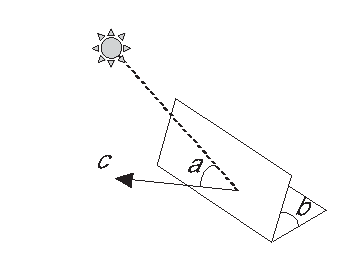
\includegraphics[width=70mm]{images/collector_theta-01.eps}
	}\hspace{1cm}
	\subfloat{
		\psfrag{S}[c][c]{S}
		\psfrag{N}[c][c]{N}
		\psfrag{a}[c][c]{$\Sigma$}
		\psfrag{b}[c][c]{$\beta$}
		\psfrag{c}[c][c]{$\phi_\textnormal{S}$}
		\psfrag{d}[c][c]{$\phi_\textnormal{C}$}
		\centering
			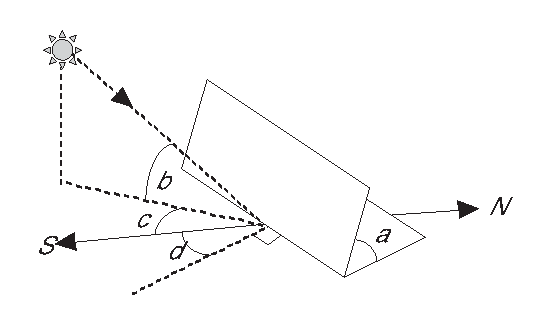
\includegraphics[width=90mm]{images/collector_geometry-01.eps}
	}
	\caption[Geometric conditions between solar irradiation and alignment of the photovoltaic panel]{Geometric conditions between solar irradiation and alignment of the photovoltaic panel \cite{masters04}}
	\label{fig:collector}
\end{figure}

% --- Electronic circuits ---
\chapter{Electronic circuits}

Use the \textbf{tikz} package to draw electronic circuits and more.

Figure \ref{fig:diode_solar_cell} shows the one diode equivalent circuit of a real solar cell.

\begin{figure}[htb]
	\centering
	\begin{tikzpicture}[
		circuit ee IEC,
		set inductor graphic=var inductor IEC graphic,
		scale = 0.85,
		]
		\draw (0,0) to [current source] (0,3);
		\draw (0,3) to [current direction={info=$I_\textnormal{Ph}$}] (2,3);
		\draw (2,3) -- (4,3);
		\draw (2,3) to [current direction={info={$I_\textnormal{D}$}}] (2,1.5) to [diode] (2,0);
		\draw (0,0) to (8,0);
		\draw (4,0) to [resistor={info={$R_\textnormal{P}$}}] (4,3);
		\draw (4,3) to [resistor={info={$R_\textnormal{S}$}}] (6,3);
		\draw (6,3) to [current direction={info={$I_\textnormal{L}$}}] (8,3);
		\draw (8,3) to [resistor={info={$R_\textnormal{L}$}}](8,0);
		\draw [->] (6,2.8) -- (6,0.2);
		\draw (6,1.5) node[anchor=west]{$U_\textnormal{L}$};
	\end{tikzpicture}
	\caption[One diode equivalent circuit of a real solar cell]{One diode equivalent circuit of a real solar cell \cite{wagner2010}}
	\label{fig:diode_solar_cell}
\end{figure}

\newpage

% Continue with roman page numbering
\pagenumbering{Roman}
\setcounter{page}{\value{romanpagenumbers}}

% Print the bibliography
\printbibliography
  
% End of document
\end{document}